\documentclass{article}

\usepackage[utf8]{inputenc}

\title{COMP 540 Assignment \#1}
\author{Yunda Jia yj32}
\date{\today}
\usepackage{natbib}
\usepackage{graphicx}
\usepackage{geometry}
\usepackage{amsmath}
\setcounter{section}{-1}
\geometry{left=2.0cm,right=2.0cm}

\begin{document}
\maketitle

\section{Background refresher(30 points)}
\begin{itemize}
	\item Plot the categorical distribution.\\
\begin{figure}[h!]
	\centering
	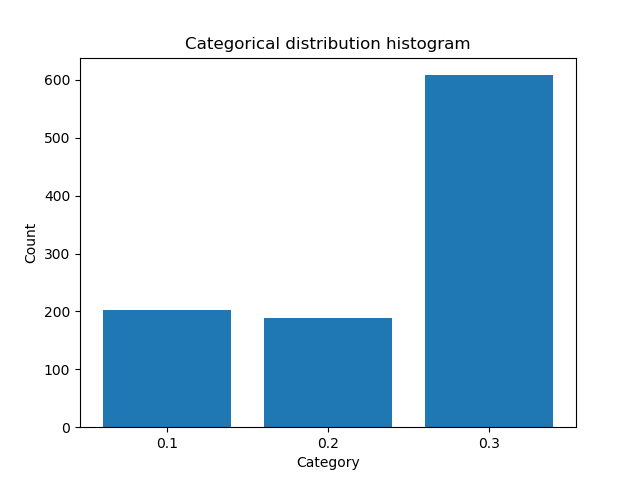
\includegraphics[scale = 0.8]{Categorical_distribution.png}
	\caption{Categorical distribution}
\end{figure}

\item Plot the Univariate normal distribution with mean of and standard deviation of 1.\\
\begin{figure}[h!]
	\centering
	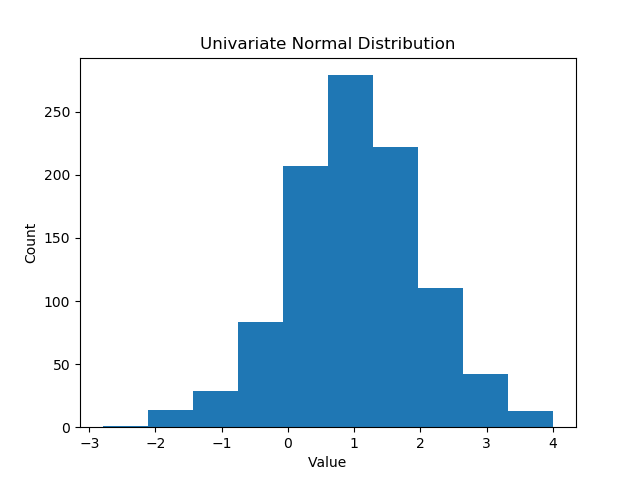
\includegraphics[scale = 0.8]{Univariate_distribution.png}
	\caption{Univariate Normal Distribution}
\end{figure}\\

\item Produce a scatter plot of the samples for a 2-D Gaussian.\\
\begin{figure}[h!]
	\centering
	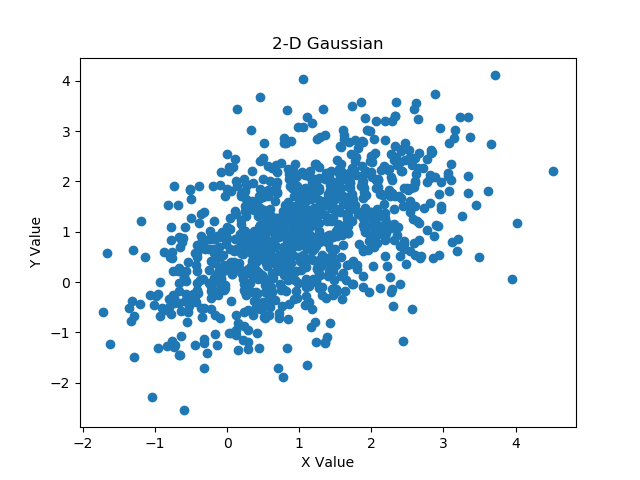
\includegraphics[scale = 0.6]{GaussianScatterPlot.png}
	\caption{Univariate Normal Distribution}
\end{figure}\\



\end{itemize}
\section{Keys, Relational Calculus and Relational Algebra}
\subsection{Keys}
\begin{enumerate}
	\item 
\end{enumerate}
\noindent\rule[0.25\baselineskip]{\textwidth}{1pt}

\end{document}